	
	\subsection*{1.}
	
	\begin{center}
		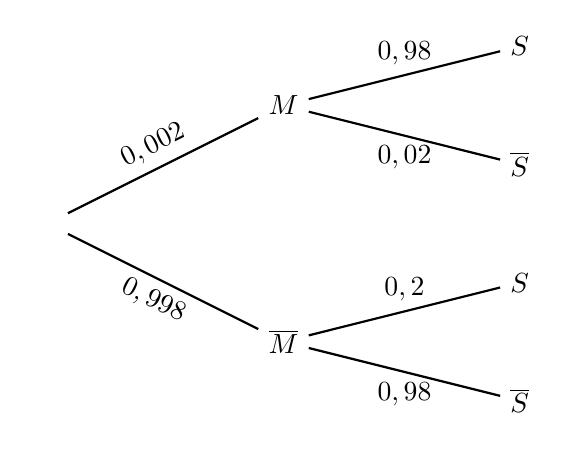
\begin{tikzpicture}[thick, scale=1.5]
			\node (P_-1_0) at (-2,-1.5) {$\phantom{A}$};
			\node (P_0_0) at (0,-0.5) {$M$};
			\draw (P_-1_0) -- (P_0_0) node[midway, above,sloped] {$0,002$};
			\node (P_1_0) at (2,-0) {$S$};
			\draw (P_0_0) -- (P_1_0) node[midway, above] {$0,98$};
			\node (P_1_1) at (2,-1) {$\overline{S}$};
			\draw (P_0_0) -- (P_1_1) node[midway, below] {$0,02$};
			\node (P_0_2) at (0,-2.5) {$\overline{M}$};
			\draw (P_-1_0) -- (P_0_2) node[midway, below,sloped] {$0,998$};
			\node (P_1_2) at (2,-2) {$S$};
			\draw (P_0_2) -- (P_1_2) node[midway, above] {$0,2$};
			\node (P_1_3) at (2,-3) {$\overline{S}$};
			\draw (P_0_2) -- (P_1_3) node[midway, below] {$0,98$};
		\end{tikzpicture}
	\end{center}
	
	On a :
	\[
	p(M) = \dfrac{1}{500} = \dfrac{2}{1000} = 0,002.
	\]
	D'où \( p(\overline{M}) = 1 - 0,002 = 0,998 \).
	
	\subsection*{2.}
	D'après la loi des probabilités totales :
	\[
	p(S) = p(M \cap S) + p(\overline{M} \cap S),
	\]
	avec :
	\begin{align*}
		p(M \cap S) &= p(M) \times p_M(S) = 0,002 \times 0,98 = 0,00196, \\
		p(\overline{M} \cap S) &= p(\overline{M}) \times p_{\overline{M}}(S) = 0,998 \times 0,02 = 0,01996.
	\end{align*}
	Donc :
	\[
	p(S) = 0,00196 + 0,01996 = 0,02192.
	\]
	
	\subsection*{3.}
	
	\paragraph{a.} Les passages étant indépendants les uns des autres et la probabilité de faire sonner étant pour chaque voyageur de \(0,02192\), \(X\) suit une loi binomiale de paramètres \(n = 2\) et \(p = 0,02192\).
	
	\paragraph{b.} Reprendre et compléter le tableau donnant la loi de \(X\) :
	
	\[
	\begin{array}{|c|c|c|c|}
		\hline
		k            & 0        & 1        & 2        \\
		\hline
		p(X = k)     & 0,95664 & 0,04288 & 0,00048 \\
		\hline
	\end{array}
	\]
	
	\paragraph{c.} On a :
	\[
	E(X) = 0 \times 0,95664 + 1 \times 0,04288 + 2 \times 0,00048 = 0,04384.
	\]
	Cela signifie qu'en moyenne, sur un grand nombre de passages, un peu plus de \(4\%\) de passagers feront sonner, alors qu'ils ne devraient être que \(0,2\%\).
	
